\documentclass{beamer}



\usepackage[utf8]{inputenc}
\usepackage[ngerman]{babel}
\usepackage{verbatim}
\usepackage{hyperref}
\usepackage{url}
\usepackage{fancyvrb}

\title{JOSM Workshop}
\author{Stefan Tiran  osm@stefantiran.at}
\date{April 27th, 2018}

\usetheme{Antibes}

%\usebackgroundtemplatei{
%\includegraphics[width=\paperwidth,
%height=0.8\paperheight]{mag_map.png}
%}

\begin{document}


\begin{frame}{Agenda}
  \begin{itemize}
    \item Erste Demo zum Kennenlernen
    \item Vorstellung des Vortragenden
    \item Kurze Einführung in das OSM--Datenmodell
    \item Kurzer Überblick über das OSM--Wiki
    \item Eingabe von Adressen
    \item Arbeiten mit Layern
    \item Arbeiten mit unterschiedlichen Datenformaten

  \end{itemize}
\end{frame}

\begin{frame}{Über den Vortragenden}

  \begin{itemize}
    \item Stefan Tiran \textless \href{mailto:osm@stefantiran.at}{osm@stefantiran.at}\textgreater
    \item IT--Entwickler an der Universität Wien
    \item Linux-User (SuSE / Ubuntu) seit 2003
    \item OpenStreetMap seit August 2008
    \begin{itemize}
      \item OSM-Username: \emph{StefanTiran}
      \item Mapping-Area: Marchfeld, Graz, Südsteiermark
    \end{itemize}
  \end{itemize}
\end{frame}

\begin{frame}[fragile]{Das OpenStreetMap--Datenmodell}

Das OSM-Datenmodell besteht aus den folgenden Elementen:
\begin{itemize}
  \item 
\includegraphics[height=0.8em]{node}\hspace{0.2em} Punkt bzw. Knoten (Englisch: node) 
  \item 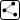
\includegraphics[height=0.8em]{way} \hspace{0.2em} 
\includegraphics[height=0.8em]{closed_way}\hspace{0.2em} Linie (Englisch: way)
  \item 
\includegraphics[height=0.8em]{area} \hspace{0.2em} Fläche (English: area) 
  \item 
\includegraphics[height=0.8em]{relation} \hspace{0.2em} Relation (English: relation) 
  \item 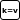
\includegraphics[height=0.8em]{tag} \hspace{0.2em} Attribut (English: tag) 

\end{itemize}

Quelle: \url{https://wiki.openstreetmap.org/wiki/DE:Elemente}

\end{frame}

\begin{frame}[fragile]{Punkt}

\begin{itemize}
  \item auch Knoten (Englisch: node)
  \item Georeferenzierter Punkt mit Längen- und Breitengrad
  \item kann Eigenschaften (Attribute) haben
  \item kann Teil eines Weges (einer Linie) sein
  \item kann Teil einer Relation sein
\end{itemize}

Quelle: \url{https://wiki.openstreetmap.org/wiki/DE:Node}

\end{frame}

\begin{frame}[fragile]{Linie}
\begin{itemize}
  \item auch Weg (Englisch: way)
  \item Sequenz von 2 - 2000 Punkten
  \item kann Punkte auch mehrfach enthalten
  \item kann dadurch offenen oder geschlossenen Linienzug darstellen
  \item hat eine Richtung
\end{itemize}

Quelle: \url{https://wiki.openstreetmap.org/wiki/DE:Way}

\end{frame}
\begin{frame}[fragile]{Fläche}

\begin{itemize}
  \item auch Fläche, Gebiet oder ausgefülltes Polygon
  \item kein eigentständiges Element im Datenmodell
  \item Modellierung als geschlossene Linie
  \begin{itemize}
    \item entweder explizit durch \texttt{area=yes} oder implizit
  \end{itemize}
  \item Modellierung als Polygon
  \begin{itemize}
    \item Typ: Multipolygon (\texttt{type=multipolygone})
  \end{itemize}
\end{itemize}
Quelle: \url{https://wiki.openstreetmap.org/wiki/DE:Area}
\end{frame}
\begin{frame}{Relation}
\begin{itemize}
  \item sortierte Liste von Datenelementen
  \item jedem Datenelement kann eine Rolle zugewiesen werden
  \item Beispiel-Typen
  \begin{itemize}
    \item Route (\texttt{type=route})
    \item Multipolygon (\texttt{type=multipolygone})
    \item Abbiegebeschränkung (\texttt{type=restriction})
   \end{itemize}
\end{itemize}
Quelle: \url{https://wiki.openstreetmap.org/wiki/DE:Relationen}
\end{frame}

\begin{frame}{Attribut}
\begin{itemize}
  \item auch Eigenschaft (Englisch: tag)
  \item besteht aus Schlüssel und Wert
  \item Der Schlüssel bestimmt die Art der Eigenschaft
  \item Der Wert beschreibt die Eigenschaft
  \item Schlüssel / Werte sind Konvention der einzelnen Communities
  \item Je zentraler ein Gebiet, desto genormter
\end{itemize}
Quelle: \url{https://wiki.openstreetmap.org/wiki/DE:Attribut}
\end{frame}

\begin{frame}{Überblick über das Wiki}
\begin{itemize}
  \item Ein passendes Attribut finden:
  \begin{itemize}
    \item \href{https://wiki.openstreetmap.org/wiki/DE:Map_Features}{DE:Map Features}
    \item \href{https://wiki.openstreetmap.org/wiki/DE:How_to_map_a}{DE:How to map a}
  \end{itemize}
  \item Ein Event eintragen, damit es auf der Hauptseite sichtbar wird: \href{https://wiki.openstreetmap.org/wiki/Template:Calendar}{Template:Calendar}
\end{itemize}
\end{frame}

\begin{frame}{Eingabe von Adressen}
\begin{itemize}
  \item Adress-Attribute sind im Namensraum \texttt{addr:} organisiert
  \item Tagging-Schema wird auch als Karlsruhe Schema bezeichnet
  \item Adresse besteht aus
  \begin{itemize}
    \item \texttt{addr:housenumber} (in UK alternativ \texttt{addr:housename}
    \item \texttt{addr:street} oder \texttt{addr:place}
    \item \texttt{addr:postcode}
    \item \texttt{addr:city} oder \texttt{addr:place}
    \item \texttt{addr:country}
  \end{itemize}
\end{itemize}
\end{frame}

\begin{frame}{Eingabe von Adressen Teil 2}
\begin{itemize}
  \item Geeignete Elemente für Adress-Attribute:
  \begin{itemize}
    \item Umrissfläche eines Gebäudes (\texttt{building=*})
    \item Punkt, der Eingang in das Gebäude kennzeichnet (\texttt{entrance=yes})
    \item Einzelpunkt, falls Gebäudeumriss nicht erruierbar
    \item POIs
    \begin{itemize}
      \item \texttt{amenity=*} Einrichtung
      \item \texttt{shop=*} Geschäfte
      \item \texttt{tourism=*} Elemente, die für Tourismus genutzt werden
    \end{itemize}
  \end{itemize}
\end{itemize}

\end{frame}

\begin{frame}{Eingabe von Adressen Teil 3}
\begin{itemize}
  \item Nützliche Plug-Ins:
  \begin{itemize}
    \item HouseNumberTaggingTool: Bequemes Erfassen einer Straße
    \item austriaaddresshelper: Automatische Abfrage der Daten vom Bundesamt für Eich- und Vermessungswesen
  \end{itemize}
\end{itemize}

\end{frame}

\begin{frame}{Arbeiten mit unterschiedlichen Datenformaten}
\begin{itemize}
  \item Öffnen selbst erfasster Daten
  \begin{itemize}
    \item .gpx (GPS-Tracks)
    \item .jpg (georeferenzierte Fotos)
  \end{itemize}
  \item Verwendung von Open Government Data
  \begin{itemize}
    \item In Österreich auf \url{https://www.data.gv.at/}  
    \item Meistens Shapefiles
    \item opendata-Plugin erforderlich
  \end{itemize}
\end{itemize}
\end{frame}

\begin{frame}
Folien zum JOSM--Workshop auf den
\href{http://http://linuxtage.at/}{Grazer Linuxtagen} am 27. 4. 2018.
\vspace{1cm}

Folien unter 
\includegraphics[width=1cm]{cc-by-sa.png}.
Icons der Datenelemente erstellt von \href{https://wiki.openstreetmap.org/wiki/User:Ck3d}{Ck3d}
\vspace{1cm}

Erstellt mittels \LaTeX Beamer, Source auf \url{https://github.com/StefanTiran/josm_ws_glt18/}.
\vspace{1cm}

\href{mailto:osm@stefantiran.at}{Stefan Tiran}
\end{frame}


\end{document}


%%:foldmethod=expr
%% vim:fde=getline(v\:lnum)=~'^%%%%\ .\\+'?'>1'\:'='
%%% Local Variables: 
%%% mode: latex
%%% mode: auto-fill
%%% mode: flyspell
%%% eval: (ispell-change-dictionary "de_AT")
%%% TeX-master: "main"
%%% End: 

